\chapter{Análisis comparativo Quorum y Fabric}
\section{Redes disponibles}
Quorum es una tecnología blockchain open source creada por J.P. Morgan e implementada sobre Ethereum, que añade diferentes mejoras a la plataforma para adaptarla al mundo financiero, aunque se puede utilizar en cualquier tipo de industria. Utiliza algoritmos de consenso distintos a Ethereum, es privada y permisionada, ya que implementa control de acceso a los nodos, y tiene un rendimiento mucho mejor que Ethereum.
Hyperledger Fabric es también open source, y fue creada por IBM y Linux Foundation. Es privada y completamente modular, lo que la ha convertido en una de las opciones mas populares a la hora de implementar soluciones empresariales.\\
Ambos tipos de tecnologías tienen ventajas y desventajas a la hora de implementar Alastria ID. En los siguientes apartados se hará una comparativa entre ambas tecnologías.
\section{Casos de uso}
Ambas redes están orientadas al entorno empresarial, por lo que los casos de uso disponibles son muy similares. Sus principales puntos fuertes son la privacidad y el rendimiento, por lo que son idóneas para utilizarse como libro de cuentas o para aumentar la transparencia de las gestiones en un grupo empresarial. También son muy adecuadas para la gestión de identidad y datos personales, gracias a las características propias de la blockchain.
\clearpage
\section{Métricas tecnológicas}
En cuanto a la comparación técnica, el funcionamiento interno de ambas tecnologías es muy distinto, pero sus métricas son similares.
\subsection*{Rendimiento y consenso}
Ambas redes, al ser privadas y permisionadas, tienen un rendimiento muy alto, debido a que no necesitan algoritmos de consenso pesados. En Quorum, se utilizan \textit{RAFT}, \textit{Proof of Authority} o \textit{Istanbul BFT} como algoritmos de consenso, mucho mas rápidos que \textit{Proof of Work}, utilizado en Ethereum. En el caso de Fabric, el algoritmo por defecto es Solo, usado únicamente en entornos de prueba, aunque al ser modular, se pueden usar otros algoritmos decididos por los miembros de cada red. Los más utilizados son \textit{Kafka} y \textit{RAFT}.
En cuanto a transacciones por segundo, según estudios realizados con redes de ambas tecnologías, \cite{fabric-benchmark} \cite{quorum-benchmark} Hyperledger Fabric es capaz de conseguir un pico mas alto de rendimiento, con mas de 800 t/s, aunque con cargas de trabajo mas significativas el rendimiento puede bajar hasta a 60 t/s. En el caso de Quorum, los picos son mas bajos, de alrededor de 170 t/s, pero se mantienen mas constantes cuando aumenta la carga de trabajo. Estos rendimientos son aproximados, y dependen en gran medida del algoritmo de consenso utilizado, las características de la red, o en el caso de Fabric, el tipo de base de datos que se utilice para el \textit{world state}.
\clearpage
\subsection*{Smart Contracts}
En lo referente a los smart contracts, hay algunas diferencias entre Quorum y Fabric, pero en general son muy similares. Los smart contracts son la lógica de negocio que se ejecuta en la blockchain y la actualiza, y dependiendo de la red, hay diferentes métodos de despliegue. En Quorum, cualquier nodo autorizado puede desplegar un smart contract en la red. \\
\begin{figure}[H]
\centerline{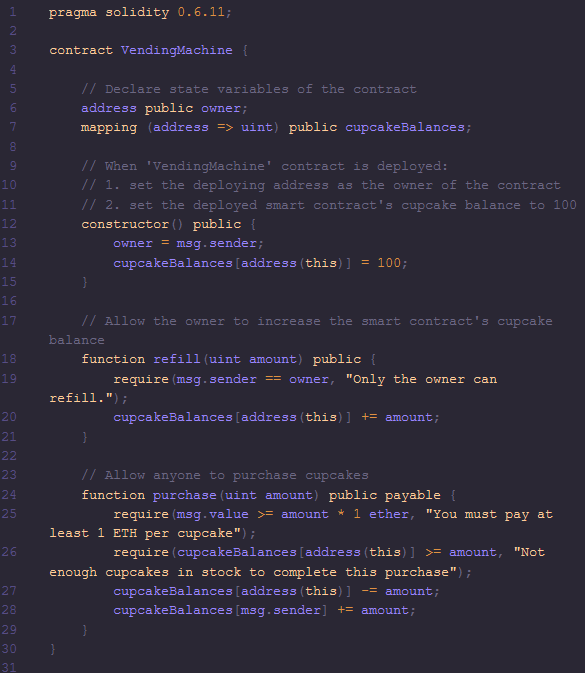
\includegraphics[scale=0.85]{recursos/smartcontracteth.png}}
\caption{Smart contract en Solidity para Ethereum \cite{SC-ETH}}
\label{sc-eth}
\end{figure}
En la imagen se puede observar un código bastante simple que permite el intercambio de ``cupcakes'' virtuales a cambio de ETH. Al ser Quorum una implementación de Ethereum, se utiliza el lenguaje Solidity para la codificación de los smart contracts de ambas tecnologías.\\

En Fabric, son las organizaciones las que despliegan el código en la red, y son las que se encargan de decidir la política de aprobación (\textit{endorsement policy}) de cada smart contract. La política de aprobación es una lista de las organizaciones cuya validación se requiere para aprobar una transacción creada por un smart contract en particular.
\begin{figure}[H]
\centerline{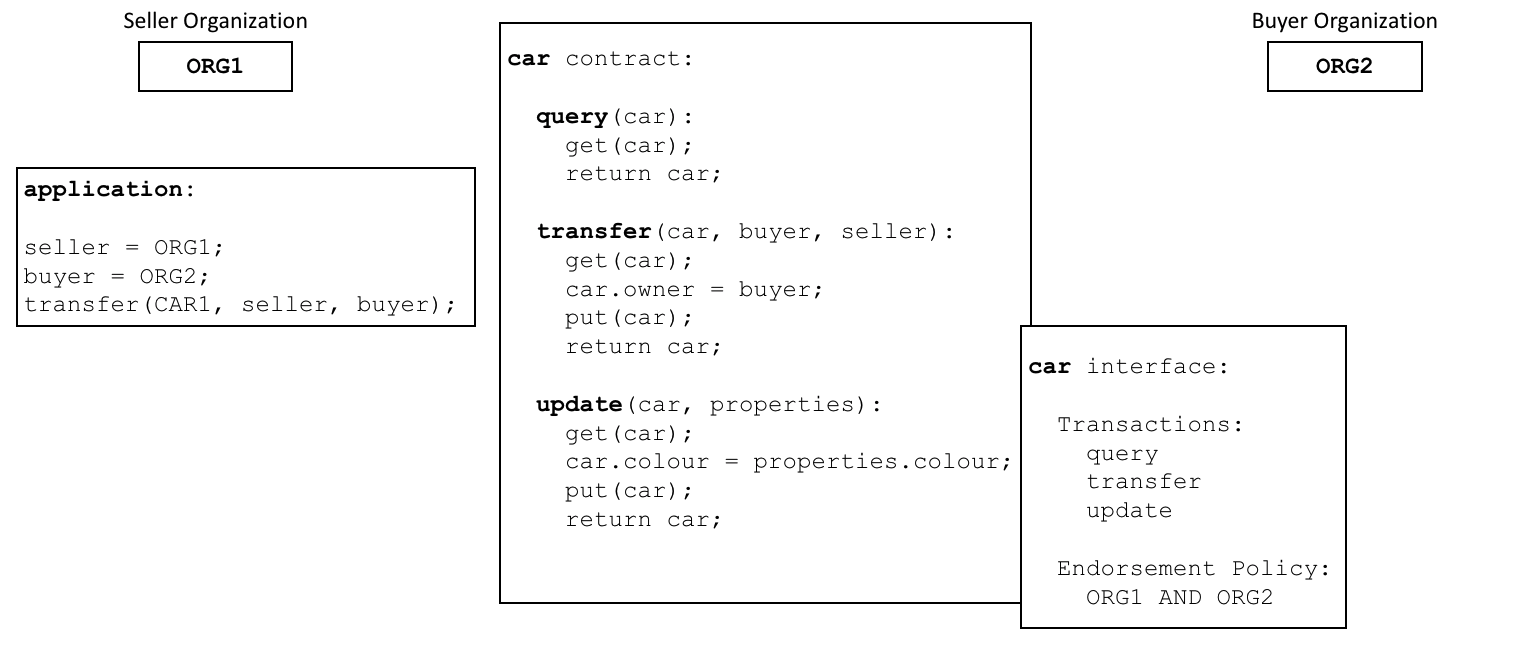
\includegraphics[scale=0.35]{recursos/SC-FABRIC-END.png}}
\caption{Smart contract de Fabric \cite{chaincodes}}
\label{sc-fabric}
\end{figure}
En la imagen se puede observar un código de un simple intercambio de objetos o \textit{assets}, con dos organizaciones involucradas, junto con su política de aprobación. Está escrito en pseudocódigo porque los smart contracts de Fabric no tienen un lenguaje único, sino que se pueden escribir en distintos lenguajes de propósito general, como Node.js o Go, lo que facilita el trabajo a desarrolladores ya experimentados. Abajo a la derecha se puede observar la política de aprobación del smart contract, que indica que organizaciones deben firmar las transacciones creadas por el smart contract para que sean válidas y puedan actualizar el world state.

Una diferencia importante entre los smart contracts de Quorum y los chaincodes de Fabric es su forma de desplegarse.
En Quorum, los smart contracts tienen su propia dirección en la red, y se comportan como un elemento más de la misma. Además, almacenan los datos en estructuras de datos implementadas en el propio código (un ejemplo es el \textit{mapping} ``cupcakeBalance'' de la figura \ref{sc-eth}). Debido a estas dos características, actualizar o mejorar el código de un smart contract desplegado es imposible, y se debe desplegar de nuevo como un contrato distinto, perdiendo asi los datos almacenados en el smart contract y cambiando su dirección. Este problema se puede solucionar con los llamados \textit{upgradeable contracts}, que permiten actualizar su código sin tener que desplegarlos de nuevo. En la implementación actual de Alastria ID para la red-T, los smart contracts no son actualizables, aunque su implementación esta en proceso.

En Fabric, los smart contracts no se despliegan por si solos, sino que se empaquetan en los chaincodes, que cada organización tiene que desplegar y aprobar para su activación en la red (por ejemplo, el smart contract de la figura \ref{sc-fabric} podría formar parte de un chaincode de vehículos mayor, con otros smart contracts como ``barco'' o ``motocicleta''). Las redes Fabric, al utilizar una base de datos de estados para almacenar los datos, no tienen problemas de perdida de información a la hora de actualizar o mejorar un chaincode, y solo con desplegar la nueva versión en la red todos los nodos involucrados apuntarán al chaincode mas actualizado.
 